\documentclass[12pt,article]{article}
\usepackage{fullpage}
\usepackage[top=2cm, bottom=4.5cm, left=2cm, right=2cm]{geometry}
\usepackage{amsmath,amsthm,amsfonts,amssymb,amscd}
\usepackage{lastpage}
\usepackage{enumerate}
\usepackage{fancyhdr}
\usepackage{mathrsfs}
\usepackage{xcolor}
\usepackage{graphicx}
\usepackage{listings}
\usepackage{hyperref}
\usepackage{mdframed}
\usepackage{changepage}   % for the adjustwidth environment
\usepackage{forest} 
\usepackage{tikz}   % For graph

\usepackage{float}  % To inforce inserting images at the right place

\newcommand{\Tau}{\mathrm{T}}


% For matrix
\def\horzbar{\text{magic}}

\hypersetup{%
  colorlinks=true,
  linkcolor=blue,
  linkbordercolor={0 0 1}
}

\setlength{\parindent}{0.0in}
\setlength{\parskip}{0.05in}

\newcommand\projnumber{1}
\newcommand\course{CS534}
\newcommand\OSUID{934370552}
\newcommand\Email{buivy@oregonstate.edu}
\newcommand\Name{Vy Bui}
\newcommand\tab[1][1cm]{\hspace*{#1}}

\pagestyle{fancyplain}
\headheight 35pt
\lhead{IA1 Competition \projnumber}
\rhead{Oct. 9, 2022}
\lfoot{}
\cfoot{}
\rfoot{\small\thepage}
\headsep 1.5em

\newenvironment{problem}[2][Problem]
    { \begin{mdframed}[backgroundcolor=gray!20] \textbf{#1 #2} \\}
    {  \end{mdframed}}
   

% Make Rightarrow with superscript
\makeatletter
\newcommand{\xRightarrow}[2][]{\ext@arrow 0359\Rightarrowfill@{#1}{#2}}
\makeatother

\begin{document}

\begin{titlepage}
    \begin{center}
        \vspace*{4cm}

        \textbf{\Large CS534 - Machine Learning}

        \vspace{0.5cm}
 
        \textbf{\Large IA1 Competition}
 
        \vspace{1cm}

        Vy Bui - 934370552

        \vspace{2cm}

        \textbf{Instructor: Dr. Xiaoli Fern}
        \vfill
             
        \vspace{0.8cm}
      
             
        The School of Electrical Engineering and Computer Science\\
        Oregon State University\\
             
    \end{center}
\end{titlepage}

%==============================================================================%
\section*{BASELINE}
The implementation from the Implementation Assignment 1, with some small 
modifications, was used as the starting point. The train data from 
\textbf{PA1\_train1.csv} was split into \textbf{training\_data} and 
\textbf{val\_data}, which comprise 80\% and 20\% of the data respectively. The 
\textbf{test\_data} is read from \textbf{PA1\_test1.csv}. All of the data was 
then normalized using $\mu_{train}$ and $\sigma_{train}$ computed from 
\textbf{training\_data}. Similar as the group IA1, date was split and ages since 
renovated was added to the feature list.

Experimented learning rates can be found in Table 1.

\begin{center}
    \begin{tabular}{ |c|c|} 
        \hline
        Learning Rate & MSE \\
        \hline
        1       & Diverge \\ 
        0.5     & Diverge \\ 
        0.15    & 4.367230 \\ 
        0.1     & 4.3682759056458 \\ 
        0.075   & 4.509987609852156 \\ 
        0.05    & 4.533113029839304 \\ 
        0.025   & 4.557692194914489 \\ 
        0.01    & 4.489928626263307 \\ 
        0.001   & 4.575720392043068 \\ 
        0.0001  & 10.808924189860564 \\ 
        \hline
    \end{tabular}
    
    Table 1: different learning rates and corresponding MSE
\end{center}

0.15 seems to yields the best model, named \textbf{$model_1$}, whose $MSE = 4.367230$
. \textbf{$model_1$} is re-trained with all of the input data. Its features' 
importance can be found in Table 2.

\begin{center}
    \begin{tabular}{ |c|c|} 
        \hline
        Feature & Weight \\
        \hline
        bias                &  5.370881 \\
        bedrooms            & -0.293320 \\
        bathrooms           &  0.349722 \\
        sqft\_living         &  0.765111 \\
        sqft\_lot            &  0.057593 \\
        floors              &  0.018585 \\
        waterfront          &  1.447041 \\
        view                &  0.575169 \\
        condition           &  0.180739 \\
        grade               &  1.121869 \\
        sqft\_above          &  0.743586 \\
        sqft\_basement       &  0.176143 \\
        yr\_built            & -0.914694 \\
        zipcode             & -0.276595 \\
        lat                 &  0.839431 \\
        long                & -0.312246 \\
        sqft\_living15       &  0.139174 \\
        sqft\_lot15          & -0.093799 \\
        month               &  0.045941 \\
        day                 & -0.054593 \\
        year                &  0.183123 \\
        age\_since\_renovated & -0.161380 \\
        \hline
    \end{tabular}
    
    Table 2: \textbf{$model_1$}'s weights
\end{center}

%================================= SECTION ====================================%
\newpage
\section*{FEATURE EXPLORATION}
Firstly, to gain some insights into the data, pandas was used to compute the 
correlations between input features and the target features (price), which are 
showned in Table 3.

\begin{center}
    \begin{tabular}{ |c|c|} 
        \hline
        Input Features & Correlation with price \\
        \hline
        id            & -0.014748 \\
        bedrooms      &  0.304994 \\
        bathrooms     &  0.524480 \\
        sqft\_living   &  0.693156 \\
        sqft\_lot      &  0.090327 \\
        floors        &  0.265757 \\
        waterfront    &  0.222654 \\
        view          &  0.392961 \\
        condition     &  0.051306 \\
        grade         &  0.671957 \\
        sqft\_above    &  0.605777 \\
        sqft\_basement &  0.295117 \\
        yr\_built      &  0.057532 \\
        yr\_renovated  &  0.095046 \\
        zipcode       & -0.048750 \\
        lat           &  0.307248 \\
        long          &  0.025544 \\
        sqft\_living15 &  0.589190 \\
        sqft\_lot15    &  0.085476 \\
        price         &  1.000000 \\
        \hline
    \end{tabular}
    
    Table 3: correlations between price and input features
\end{center}

The top three features with highest correlation with "price" are "sqft\_living", 
"grade", and "sqft\_above", from highest to lowest.
The correlation between "long" and "price" is quite small, which is reasonable 
because all of samples are houses located in Seattle, whose longitudes are very 
close to each other. This might indicate that "long" is not quite useful to 
predict the house price. However, training without using "long" results in 
worse models.

\begin{figure}[H]
    \centering
    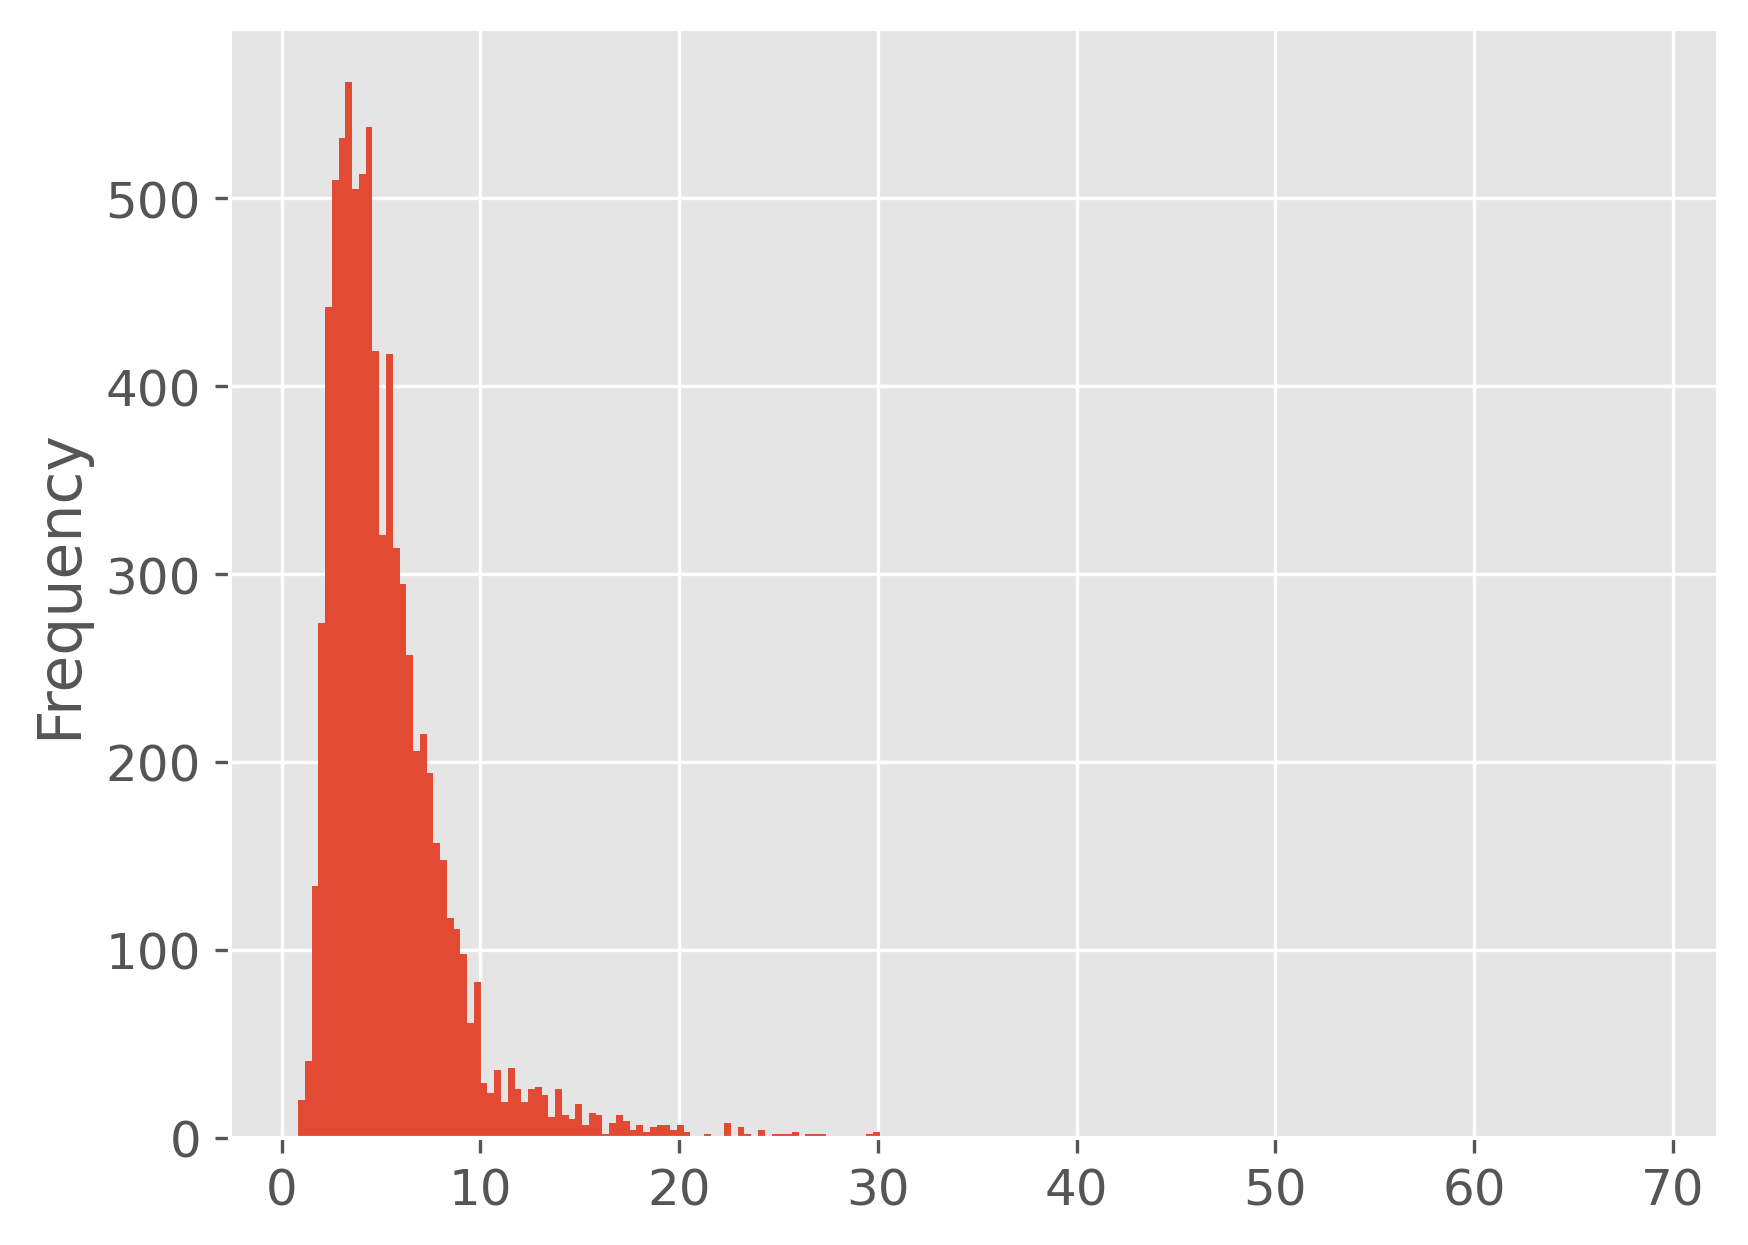
\includegraphics[scale=0.6]{price_dist.png} \par
    \caption{Histogram of price}
    \label{fig:price_hist}
\end{figure}

The house prices mainly fall in the range from [0.82,14.4], with more than 97\%, 
as showned by Figure \ref*{fig:price_hist}.
Suspecting that the outliers might negatively affect the model, I dropped the 
input data with prices $> 14.4$ to train $model_2$. It performs worse than 
$model_1$, having $MSE = 5.28$.

\newpage
The correlations between price and preprocessed input features are shown in 
Table 4.

\begin{center}
    \begin{tabular}{ |c|c|} 
        \hline
        Preprocessed Input Features & Correlation with price \\
        \hline
        bedrooms             &  0.304994 \\
        bathrooms            &  0.524480 \\
        sqft\_living          &  0.693156 \\
        sqft\_lot             &  0.090327 \\
        floors               &  0.265757 \\
        waterfront           &  0.222654 \\
        view                 &  0.392961 \\
        condition            &  0.051306 \\
        grade                &  0.671957 \\
        sqft\_above           &  0.605777 \\
        sqft\_basement        &  0.295117 \\
        yr\_built             &  0.057532 \\
        zipcode              & -0.048750 \\
        lat                  &  0.307248 \\
        long                 &  0.025544 \\
        sqft\_living15        &  0.589190 \\
        sqft\_lot15           &  0.085476 \\
        price                &  1.000000 \\
        month                & -0.008468 \\
        day                  & -0.024775 \\
        year                 &  0.001692 \\
        age\_since\_renovated  & -0.099004 \\
        \hline
    \end{tabular}
    
    Table 4: correlations between price and preprocessed input features
\end{center}


\section*{CONCLUSION}
First, $model_1$ appears to be the best model with the MSE of 4.37. Second, 
using random data split into train and validation set can result in models with 
significantly different performance. 

\end{document}
